\section{ТЕОРЕТИЧЕСКИЕ СВЕДЕНИЯ}

WCF~---~это технология для построения распределенных приложений.

Ключевым понятием в WCF является служба.
В основе своей служба~---~это множество оконечных точек (endpoints),
которые предоставляет клиентам некие полезные возможности.
Оконечная точка~---~это сетевой ресурс, которому можно посылать сообщения.
Чтобы воспользоваться предоставляемыми возможностями, 
клиент посылает сообщения оконечным точкам в формате,
который описывается контрактом между клиентом и службой.
Службы ожидают поступления сообщений на адрес оконечной точки,
предполагая, что сообщения будут записаны в оговоренном формате.

Чтобы клиент мог передать службе осмысленную информацию, он
должен знать адрес, привязку и контракт.

\textbf{Адрес} (Address, A) определяет, куда следует отправлять сообщения,
чтобы оконечная точка их получила. В случае протокола HTTP адрес будет
выглядеть так: http://myserver/myservice/.

\textbf{Привязка} (Binding, B) определяет канал для коммуникаций с оконечной
точкой. По каналам передаются все сообщения, циркулирующие в приложении
WCF. Канал состоит из отдельных элементов привязки (binding element),
которые определяют транспортный механизм, способ кодирования данных,
способы обеспечения безопасности и др. WCF позволяет заменять данные
модули на другие (например, протокол HTTP заменить на TCP) и при этом
логика приложения не изменится.

\textbf{Контракт} (Contract, C) определяет набор функций, предоставляемых
оконечной точкой, то есть операции, которые она может выполнять, и форматы
сообщений для этих операций. Описанные в контракте операции отображаются
на методы класса, реализующего оконечную точку, и включают, в частности,
типы параметров, передаваемых каждому методу и получаемых от него.
WCF-служба может состоять из нескольких оконечных точек, каждая из
которых описывается собственным адресом, привязкой и контрактом.
Поскольку поток сообщений обычно двунаправленный, клиенты не явно также
оказываются контейнерами оконечных точек.

На рисунке~\ref{pic:wcf_components} показаны компоненты, принимающие участие в коммуникациях WCF.

\begin{figure}[h!]
  \centering
  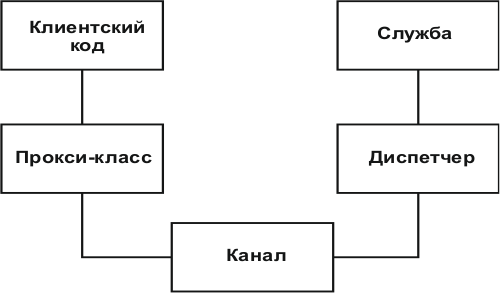
\includegraphics[width=92mm]{pic/wcf_components}
  \caption{Компоненты WCF}
  \label{pic:wcf_components}
\end{figure}

Клиент вызывает какой-либо метод прокси-класса.
Прокси-класс предлагает методы, предоставляемые службой,
но их вызов преобразуется в сообщение, которое затем передается по каналу. 
Канал имеет клиентскую и серверную части, 
взаимодействующие между собой через сетевой протокол. 
Из канала сообщение передается диспетчеру, 
который преобразует его обратно в вызов метода,
после чего указанный метод вызывается в службе.

В WCF поддерживается несколько коммуникационных протоколов:
SOAP, WSDL (Web Services Description Language~---~язык описания веб-служб),
REST (Representational State Transfer~---~передача репрезентативного состояния)
JSON (JavaScript Object Notation~---~представление объектов JavaScript).